\documentclass[UTF8]{ctexbeamer}
\usepackage{beamerthemesplit} % 加载主题宏包
\usetheme{Ilmenau} % 选用该主题
\usepackage{subfigure}
\usepackage{amsmath,amsthm,amssymb,amsfonts}
\usepackage{amsfonts,booktabs}
\usepackage{amsmath}
\usepackage{lmodern,textcomp}
\usepackage{color}
\usepackage{tikz}
\usepackage{natbib}
\usepackage{multicol}
\usepackage{caption}
\usepackage{listings}
\usepackage{ctex}
\usepackage{graphicx}

% 用来设置附录中代码的样式
\title{大学物理知识串讲(二)}
\author{谢悦晋}
\institute[Huazhong University of Science and Technology]{提高2201班\\
	u202210333@hust.edu.cn}
\date{\today}
\begin{document}
\begin{frame}
\titlepage
\end{frame}


\begin{frame}
\frametitle{小广告}
问问题和找试卷的群
\begin{figure}[!ht]
	\centering
	\begin{minipage}{.49\textwidth}
		\begin{figure}[!ht]
				\centering
				
\includegraphics[width=.9\textwidth]{37}
		\end{figure}
	\end{minipage}
		\begin{minipage}{.49\textwidth}
		\begin{figure}[!ht]
			\centering
			
\includegraphics[width=1\textwidth]{38}
		\end{figure}
	\end{minipage}
\end{figure}
\end{frame}

\section{波动}
\begin{frame}[t]
\frametitle{基本定义}
\begin{itemize}
	\item 波的分类:机械波与电磁波,横波纵波与混合波
	\item 波动方程:
	$$y=A\cos[\omega(t-\frac xu)+\varphi]=A\cos[\omega t-2\pi \nu/\lambda+\varphi]=A\cos[\omega t-kx+\varphi]$$
	\item 波长$\lambda$
	\item 周期$T$,频率$\nu$:$T_{\text{波动}}=T_{\text{振动}}$
	\item 波速$u=\dfrac{\lambda}{T}$
	\item 波数$k=\frac{2\pi}\lambda=\frac{2\pi}{uT}=\frac\omega u$:在波的传播方向上$2\pi$长度内包含的波长的个数
	\item 波的传播方向:左行波与右行波
\end{itemize}
\end{frame}

\begin{frame}[t]
\frametitle{波动方程的求法}
\begin{block}{核心思想}
	任意点P$t$时刻的位相=参考点$t-\Delta t$时刻的位相	
\end{block}
\begin{examples}
	一平面简谐波在媒质中以速度u传播,其传播路径上 P 点的振动方程为$y_p=A\cos\omega t$,试按照下图中所选择的几种坐标写出波动表达式。(P点与O点距离为L)。	
\end{examples}
\begin{figure}[!ht]
	\centering
	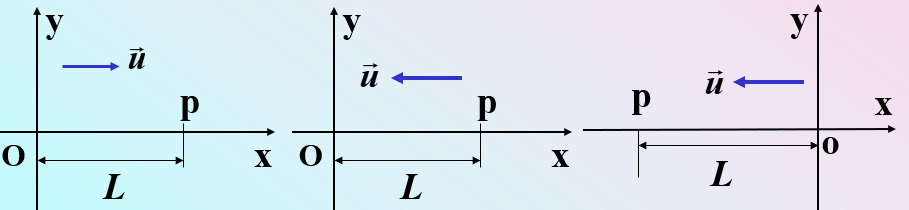
\includegraphics[width=0.9\textwidth]{1}
\end{figure}

\end{frame}



\begin{frame}
\frametitle{波的能量}
结论:
1.每一质元$\Delta m$的总能量是时间和位置的函数!
	——能量也以速度$u$随波一起传播
	\begin{align*}
		\Delta W_k&=\frac12\Delta m(\frac{\partial y}{\partial t})^2=\frac12\rho\Delta V\omega^2A^2\sin^2(\alpha t-kx+\varphi)\\
		{\Delta W}_{p}&=\frac12\Delta V\rho\omega^2A^2\sin^2(\omega t-kx+\varphi)=\Delta W_k\\
		\Delta W&=\Delta W_{k}+\Delta W_{p}=\rho\Delta V\omega^{2}A^{2}\sin^{2}(\omega t-kx+\varphi)
	\end{align*}
	固定$x$:	$W_k= W_p$
	
	固定$t$: $W_k,W_p$随x周期分布,$y = 0,W_k= W_p$最大,$y$最大$W_k,W_p$为0
\end{frame}

\begin{frame}
\frametitle{波的能量}
\begin{figure}[!ht]
	\centering
	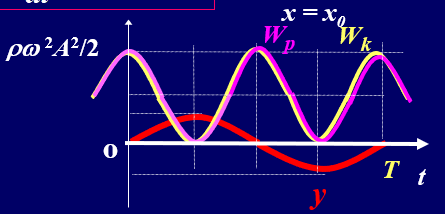
\includegraphics[width=0.5\textwidth]{2}
\end{figure}
\begin{figure}[!ht]
	\centering
	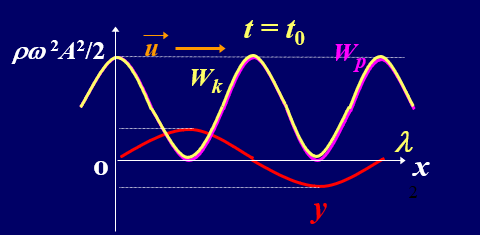
\includegraphics[width=0.5\textwidth]{3}
\end{figure}

\end{frame}
\begin{frame}
	\frametitle{波的能量}
2.质元$\Delta m$的动能和势能\textbf{同相变化},而且始终具有相同数值,质元在平衡位置时,具有最大能量
\begin{examples}
	\begin{figure}[!ht]
		\centering
		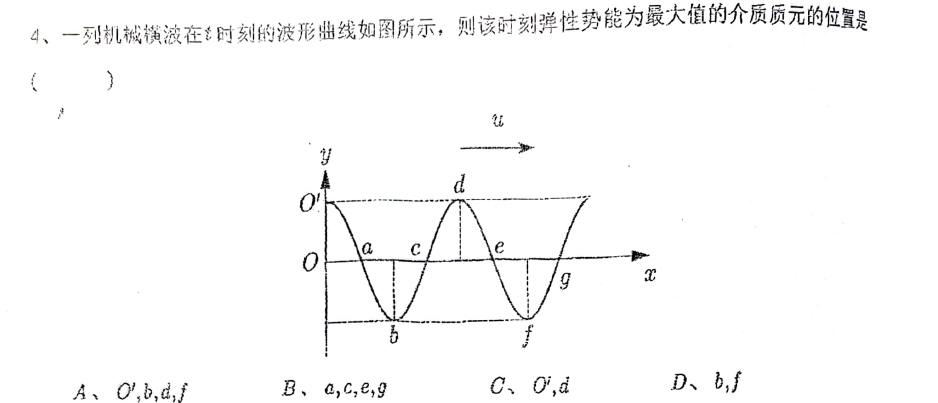
\includegraphics[width=0.8\textwidth]{4}
	\end{figure}
\end{examples}
\end{frame}
\begin{frame}
	\frametitle{波的能量}
几个有关波能量的公式(应该不会考):\\
\begin{itemize}
	\item 能量密度: 媒质单位体积内的能量
	$$w=\frac{\Delta W}{\Delta V}=\rho\boldsymbol{\omega}^2A^2\sin^2(ot-kx+\varphi)$$
	\item 能流密度: 单位时间通过垂直传播方向的单位截面上的能量
	$$i=wu=\rho\omega^2A^2u\sin^2(\omega t-kx+\varphi)$$
	\item 波的强度: 平均能流密度
	$$\begin{aligned}I=<i>=\frac1T\int_0^Tidt=\frac12\rho\omega^2A^2u \propto A^2\end{aligned}$$
\end{itemize}
\end{frame}

\begin{frame}
\frametitle{惠更斯原理}
内容:媒质中任一波阵面上的各点,都可以看作是发射子波的波源,其后任一时刻,这些子波的包迹就是新的波阵面(没考过,掌握课件中的几个例子应该足够了)
\begin{examples}
	\begin{figure}[!ht]
		\centering
		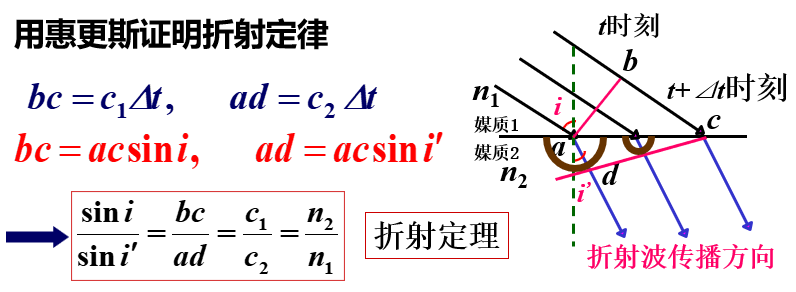
\includegraphics[width=0.8\textwidth]{5}
	\end{figure}
\end{examples}
\end{frame}


\begin{frame}
\frametitle{波的叠加与干涉}
	波的叠加原理:在几列波相遇的区域中,质元的振动是各个波单独在该点产生的振动的合成。(空间不同位置处各质元振动的叠加)
	
	波叠加的特例:波的干涉
	
	稳定干涉产生的条件(相干条件):
	相干波源发出的波在空间相遇时产生干涉,相干波源必满足
	\begin{itemize}
		\setlength{\itemsep}{0pt}
		\setlength{\parsep}{0pt}
		\setlength{\parskip}{0pt}
		\item \textbf{频率相同}
		\item \textbf{振动方向相同}
		\item \textbf{相位差恒定}
	\end{itemize}
	两波源的相同方向振动的\textbf{振幅相近或相等}时干涉现象明显。
\end{frame}
\begin{frame}
	\frametitle{波的干涉}
\begin{block}{重要公式}
	波源$S1:y_1=A_1\cos(\omega t+\varphi_1),S2:y_2=A_2\cos(\omega t+\varphi_2)$,任意点P的振动方程:$y_p=y_{1p}+y_{2p}=A\cos(\omega t+\varphi)$,其中:
	$$\begin{aligned}A^2&={A_1}^2+{A_2}^2+2A_1A_2\cos \Delta\phi\\
	\Delta\phi&=\phi_2-\phi_1=-\frac{2\pi(r_2-r_1)}\lambda+\varphi_2-\varphi_1\end{aligned}$$
\end{block}
\begin{itemize}
	\item $\Delta\phi=\pm2n\pi $振动加强
	\item $\Delta\phi=\pm(2n+1)\pi $振动减弱
\end{itemize}
\end{frame}
\begin{frame}
\frametitle{波的干涉}
\begin{examples}
	两波源B和D具有相同的振动方向和振幅,$\varphi_D-\varphi_B=\pi$,其发出的两列平面简谐波沿相反方向传播。频率均为100Hz,波速400ms$^{-1}$。B在坐标原点处,BD=30m。求(1)两波源的振动方程。(2)BD连线上因干涉而静止的点的位置。
	\begin{figure}[!ht]
		\centering
		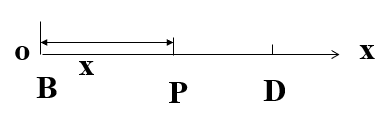
\includegraphics[width=0.5\textwidth]{6}
	\end{figure}
\end{examples}
  \end{frame}
\begin{frame}
	\frametitle{波的干涉}
		\begin{figure}[!ht]
			\centering
			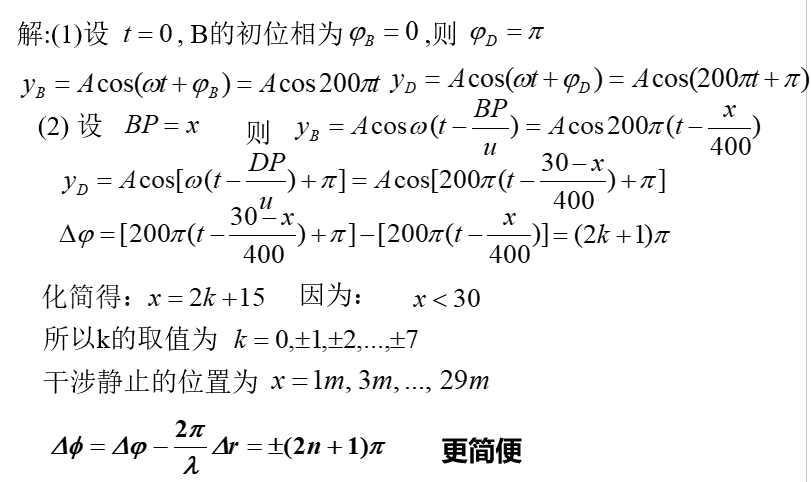
\includegraphics[width=0.9\textwidth]{7}
		\end{figure}
\end{frame}
\begin{frame}
\frametitle{驻波}
定义:两列振幅相等的相干波相向而行,在相遇的区域迭加干涉,形成驻波.
		\begin{figure}[!ht]
	\centering
	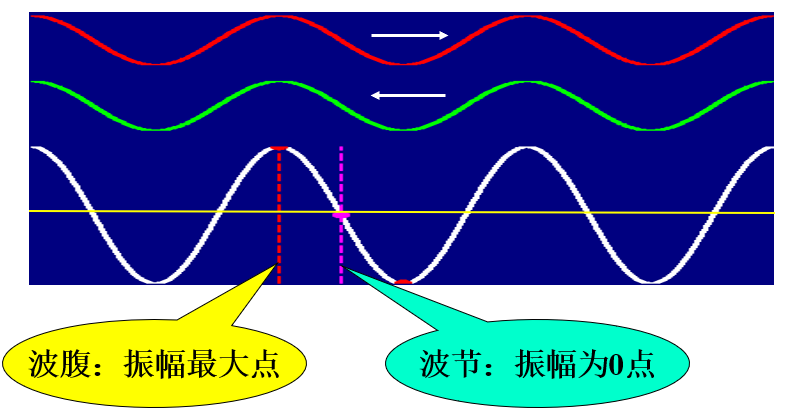
\includegraphics[width=0.9\textwidth]{8}
\end{figure}
\end{frame}
\begin{frame}
\frametitle{驻波}
\begin{block}{驻波方程}
	设两列波为平面余弦波$y_1=A\cos\omega(t-\frac xu),y_2=A\cos\omega(t+\frac xu)$,则合成波:$y=y_1+y_2=2A\cos\frac\omega ux\cdot\cos\omega t$, 其中$A_{\text{驻}}=2A\cos\frac\omega ux$描述每个固定点的振幅
\end{block}
\begin{itemize}
	\item 波腹位置:$A_{\text{驻}}=2A,x=\pm(2n+1)\frac\lambda4$
	\item 波节位置:$A_{\text{驻}}=0,x=\pm n\frac\lambda2$
	\item 驻波的位相关系:相邻波节之间的各点同相,任一波节
	两侧的质点反相.
\end{itemize}
振动状态不传播,因此驻波中没有净能量传递,能流密度为0。波形不动,分段振动(故而‘驻’波)
\end{frame}
\begin{frame}
\frametitle{驻波中的半波损失}
		\begin{figure}[!ht]
	\centering
	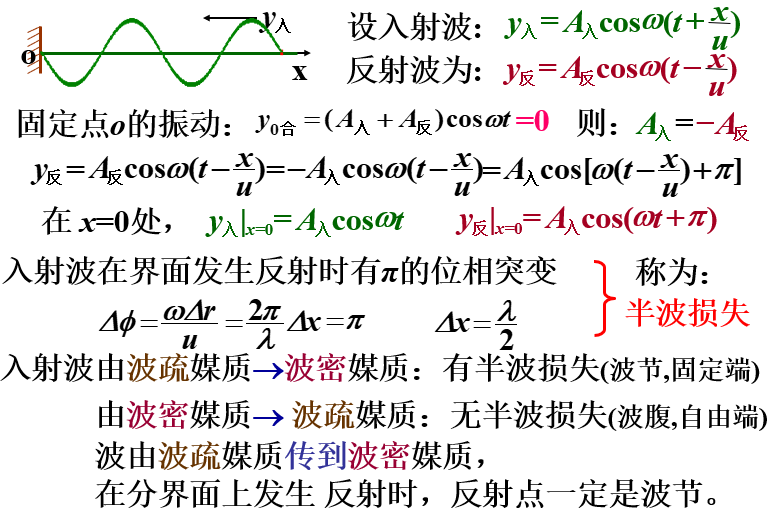
\includegraphics[width=0.9\textwidth]{9}
\end{figure}
\end{frame}
\begin{frame}
\frametitle{驻波}
\begin{examples}
	平面简谐波$y=A\cos(\omega t-kx)$在$x_0=4\lambda$处(固定端)反射,求(1)反射波的波函数;(2)驻波的波函数;(3)0与$x_0$处之间的各个波节和波腹的位置。
			\begin{figure}[!ht]
		\centering
		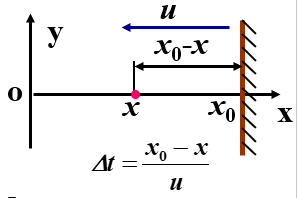
\includegraphics[width=0.5\textwidth]{10}
	\end{figure}
\end{examples}
\end{frame}
\begin{frame}
	\frametitle{多普勒效应}
				\begin{figure}[!ht]
		\centering
		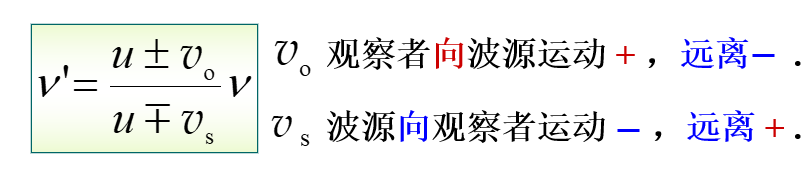
\includegraphics[width=0.9\textwidth]{11}
	\end{figure}
	\begin{examples}
		A、B 为两个汽笛,其频率皆为500Hz,A 静止,B 以60m/s 的速率向右运动. 在两个汽笛之间有一观察者O,以30m/s 的速度也向右运动. 已知空气中的声速为330m/s,求:(1)观察者听到来自A 的频率(2)观察者听到来自B 的频率(3)观察者听到的拍频
	\end{examples}
\end{frame}
\begin{frame}
\frametitle{电磁波与电磁振荡}
给定电场波动方程会求磁场方程,反之一样

$\vec{E},\vec{H}$的变化是同步的,位相相同,数量(幅值)关系为:
$$\sqrt{\boldsymbol{\varepsilon}}E=\sqrt{\boldsymbol{\mu}}H$$

$\vec{E}\bot\vec{H}\bot\vec{u}$, $\vec{E}\times\vec{H}$ 的方向就是$u$的方向$\vec{E}$ $\vec{H}$ 在各自的平面上振动,是横波
\begin{examples}
	已知 $H_x=-H_0\cos\omega(t+\frac{{Z}}c),H_y=H_z=0$  写出 $\vec{E}$ 的波动方程
	
	已知 $E_y=800\cos\omega(t+\frac xc),E_x=E_Z=0$ 写出$\vec{H}$ 的波动方程
\end{examples} 
\end{frame}
\section{光学}
\begin{frame}
\frametitle{基本概念}
\begin{itemize}
	
	\item 光程: $r=\sum n_iL_i$
	
	\item 光程差: $\Delta r=n_2L_2-n_1L_1$
	
	\item 透镜或透镜组在光路中不会带来附加的光程差。
	
	\item 光的相干条件
	
	\item 半波损失:光疏介质到光密介质的反射存在半波损失,光密介质到光疏介质的反射无半波损失
	
	\item \textbf{出题角度:光强分布,明暗纹条件和位置,动态变化,斜入射}
\end{itemize}
\end{frame}
\begin{frame}
\frametitle{杨氏双缝干涉}
				\begin{figure}[!ht]
	\centering
	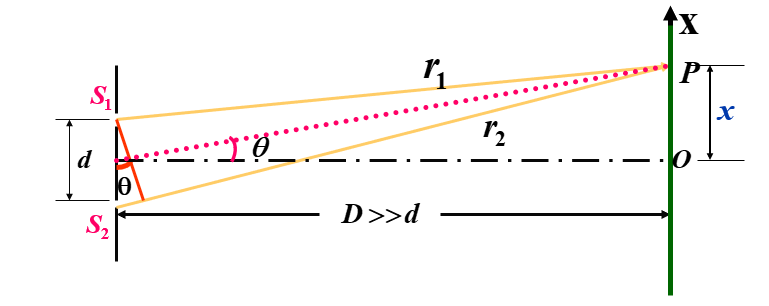
\includegraphics[width=0.7\textwidth]{12}
\end{figure}
\begin{block}{结论}
	$\Delta r=d\sin\theta=d\frac{X}{D}=\begin{cases}\quad k{\lambda}&\text{,明纹}\\(2k+1)\frac{\lambda}{2}&\text{,暗纹}\end{cases}\quad k=0,\pm1,\pm2,...$
	
	相邻两条明(暗)纹的间距: $\quad{\Delta x=\frac Dd\lambda}$
	
	光强分布:$I_\alpha=I_0\cos^2\alpha\quad,\quad\alpha=\dfrac{\pi d\sin\theta}\lambda$
\end{block}
\end{frame}
\begin{frame}
\frametitle{杨氏双缝干涉}
动态变化的分析
\begin{itemize}
	\item $D,\lambda$ 一定, $\Delta x\propto \frac1d,d\downarrow,\Delta x\uparrow$条纹越清晰
	\item $D\text{、}d$ 一定,$x_k\propto\lambda$,同一级上 $\lambda\uparrow,x_k\uparrow$(中央极大除外)
\end{itemize}
\begin{examples}
	缝间距d=1.00mm的杨氏实验中,缝屏到屏幕间的距离为D=10.00m。屏幕上条纹间隔为$4.73\times 10^{-3}$m。问入射光的频率为多少?实验在水中进行$n_w=1.333$
\end{examples}
\begin{examples}
	杨氏实验中,入射光的波长为6000埃,当把一个厚度为t=1mm的薄膜放在光源S1处,发现中央条纹移到第七个亮纹的位置,求薄膜的折射率。
\end{examples}
\end{frame}
\begin{frame}
\frametitle{杨氏双缝干涉}
\begin{examples}
	\begin{figure}[!ht]
		\centering
		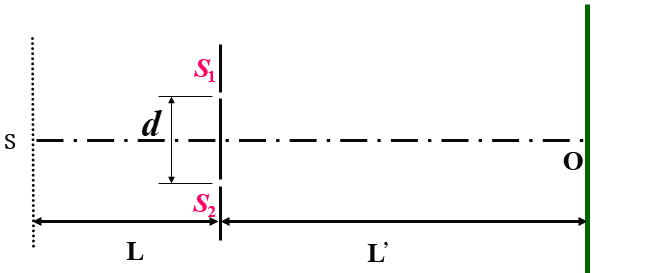
\includegraphics[width=0.6\textwidth]{13}
	\end{figure}
	(1)光源S向上移动 $l$,干涉图案向何方移动多少?
	
	(2)光源S逐渐变为较长波长的单色光,干涉图样怎么变化?
	
	(3)两狭缝距离2d,干涉图样中相邻极大之间的距离怎么变化?
	
	(4)两光源的光分别通过各自的狭缝,干涉图样是什么样的?
	
	(5)两狭缝自身宽度加倍,干涉图样相邻极大间距如何变化?
\end{examples}
\end{frame}
\begin{frame}
	\frametitle{杨氏双缝干涉}
	\begin{examples}
		\begin{figure}[!ht]
			\centering
			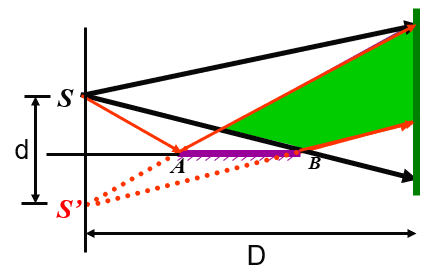
\includegraphics[width=0.5\textwidth]{14}
		\end{figure}
		洛埃镜实验中,等效缝间距d=2.00mm,缝屏与屏幕间距为D=5.00m,入射光频率$6.522\times10^{14}$Hz,实验在空气中进行,求第一级极大的位置。
	\end{examples}
\end{frame}
\begin{frame}
\frametitle{等倾干涉}
\begin{figure}
	\begin{minipage}{0.39\textwidth}
			\centering
			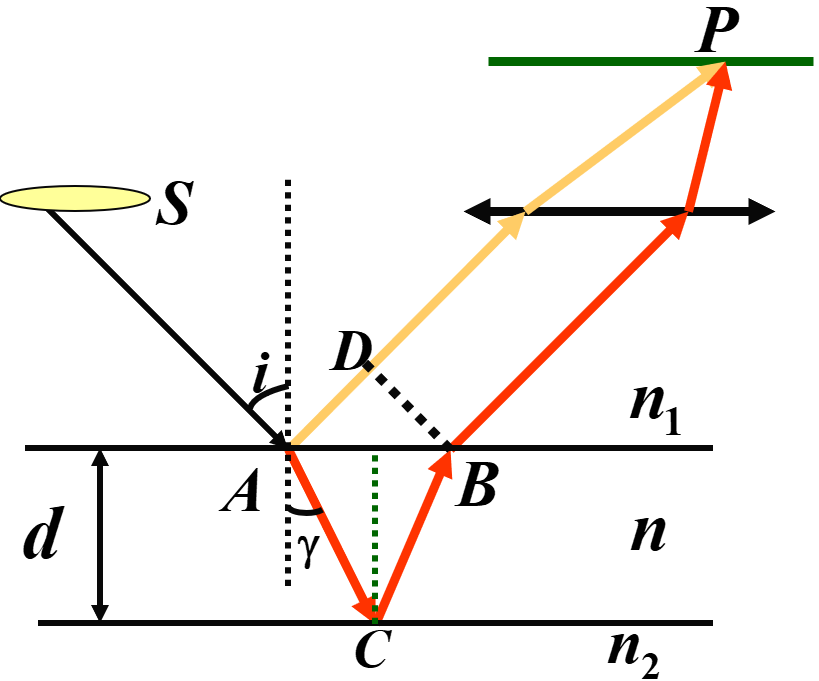
\includegraphics[width=1\textwidth]{15}
	\end{minipage}
	\begin{minipage}{0.59\textwidth}
		\begin{block}{结论}
			$ n_1<n<n_2$
			$2d\sqrt{n^2-n_1^2\sin^2i}=\begin{cases}\quad k\lambda\text{,明}\\(2k+1)\frac\lambda2\text{,暗}\end{cases} $
		\end{block}
	\end{minipage}
\end{figure}
\begin{figure}[!ht]
	\centering
	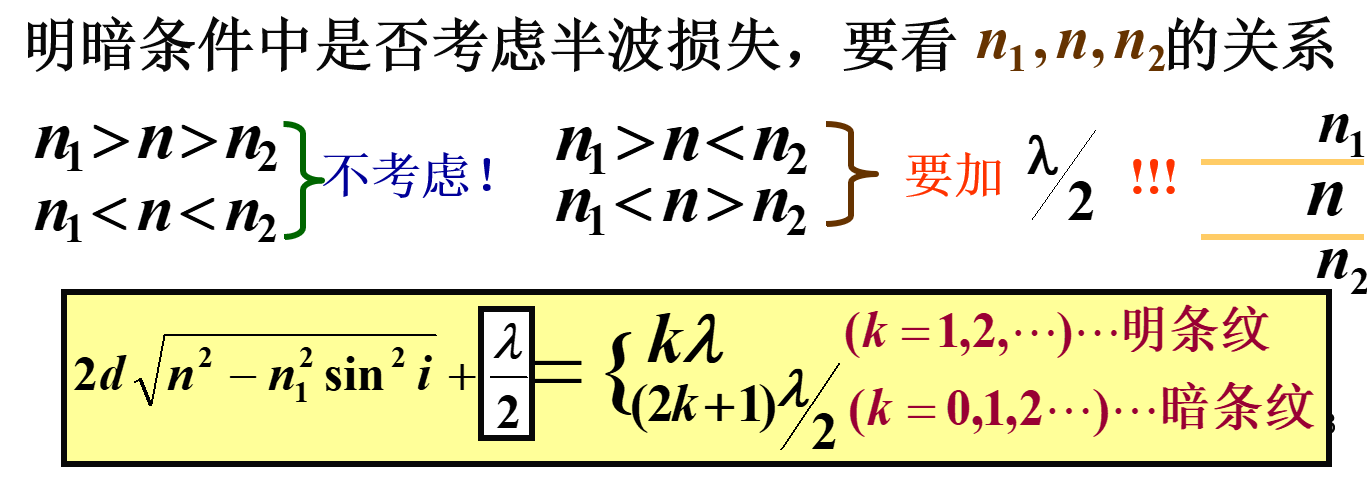
\includegraphics[width=0.8\textwidth]{16}
\end{figure}
\end{frame}

\begin{frame}
	\frametitle{条纹特征以及动态变化}
	\begin{figure}[!ht]
		\centering
		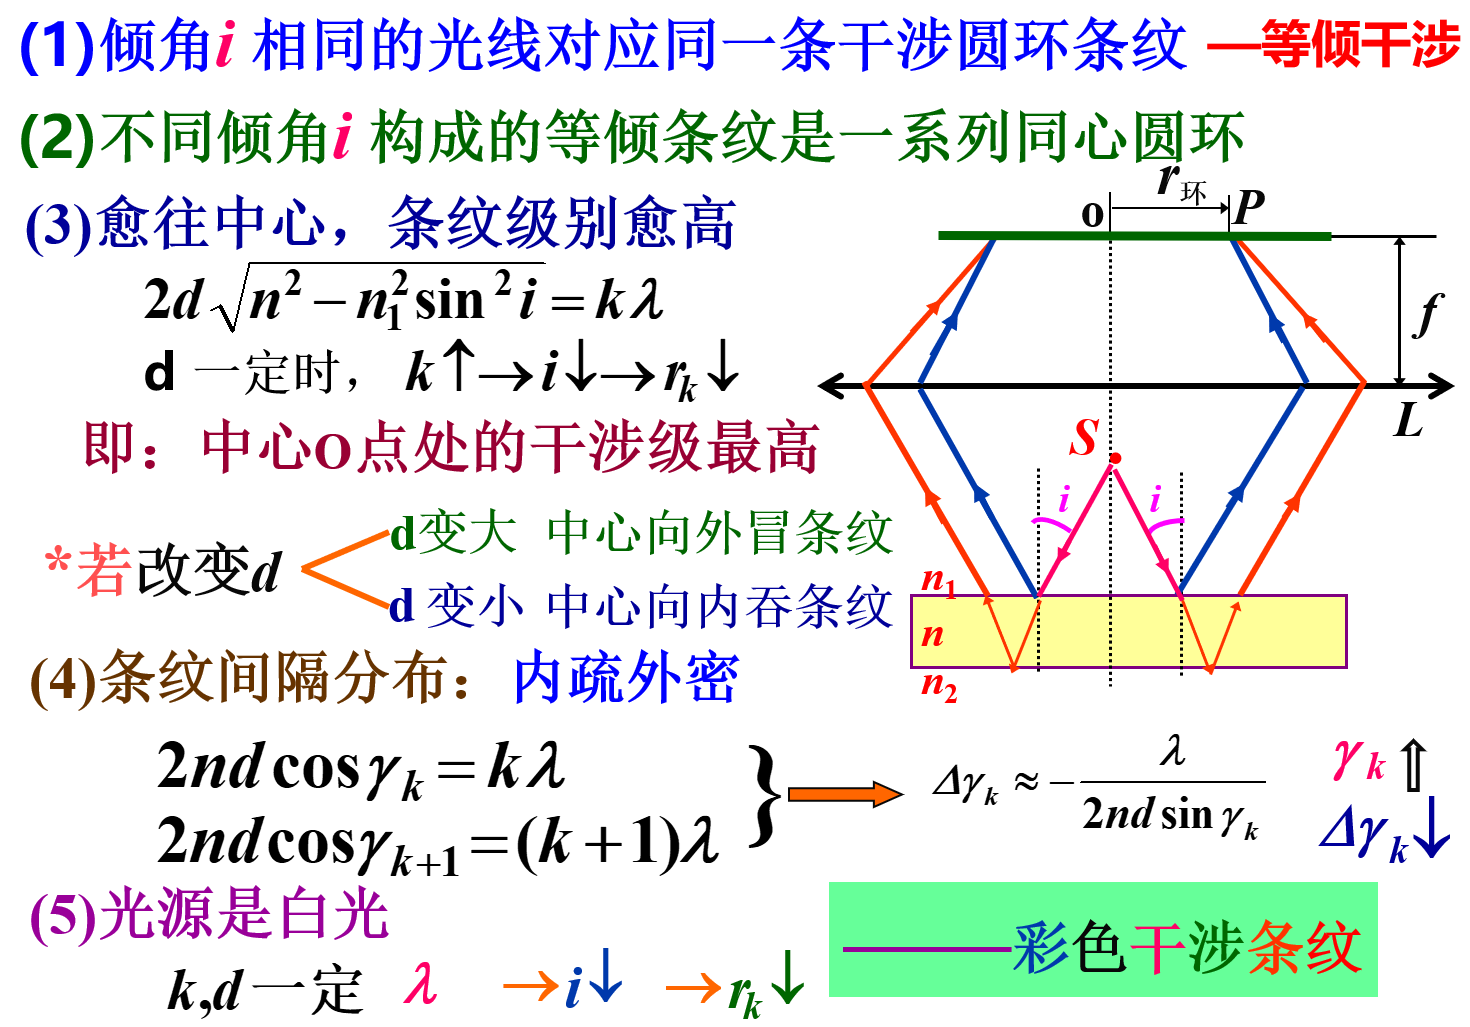
\includegraphics[width=0.8\textwidth]{17}
	\end{figure}
\end{frame}
\begin{frame}
	\frametitle{等倾干涉的几点说明}
\begin{itemize}
	\item 平行光垂直入射的干涉现象: 单色光垂直入射时, 薄膜表面或全亮、或全暗、或全居中。复色光垂直入射时,薄膜表面有的颜色亮,有的消失
	\item 透射光也有干涉现象
\end{itemize}
\begin{examples}
	折射率 n=1.50的玻璃表面涂一层 MgF$_2$(n=1.38),为使它在 5500Å波长处产生极小反射,这层膜应多厚?
\end{examples}
\begin{examples}
	空气中有一透明薄膜 $d=0.4\mu m$,$n=1.5$ 白光垂直照射。求反射光呈什么颜色?
\end{examples}
\end{frame}
\begin{frame}
	\frametitle{等厚干涉/劈尖}
	\begin{figure}[!ht]
		\centering
		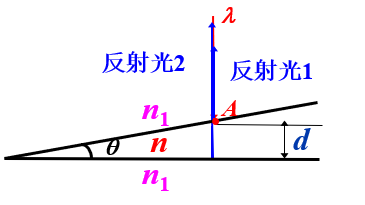
\includegraphics[width=0.5\textwidth]{18}
	\end{figure}
	\begin{block}{结论}
		$\delta=2nd+\frac\lambda2=\begin{cases}\quad k\lambda,k=1,2...\text{ ,明纹}\\(2k+1)\frac\lambda2, k=0,1...\text{,暗纹}&\end{cases}$
		
		相邻两明(暗)纹之间的厚度差:${\Delta d=\frac\lambda{2n}}$条纹间距:${L=\frac\lambda{2n\sin\theta}}$
	\end{block}
\end{frame}
\begin{frame}
	\frametitle{等厚干涉/劈尖的动态变化}
	\begin{figure}[!ht]
		\centering
		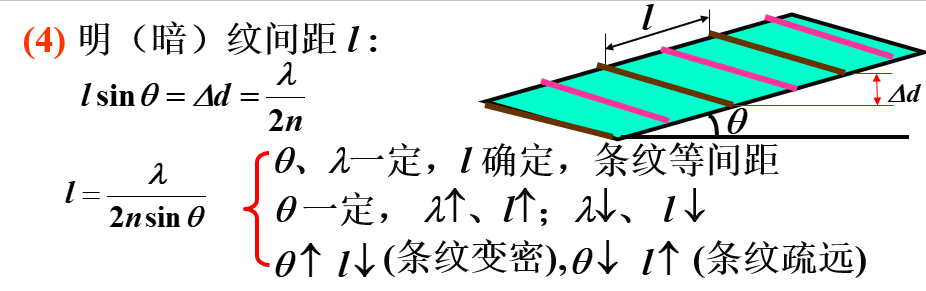
\includegraphics[width=1\textwidth]{19}
	\end{figure}
\end{frame}
\begin{examples}
	下图是检测精密加工后的工件表面光洁度的装置示意图。下面是待测工件,上面是标准平板玻璃,其间形成空气劈,用单色光垂直入射,若在反射光中观察到图示的条纹,试对工件表面的光洁度进行分析。
	\begin{figure}
		\centering
		\subfigure{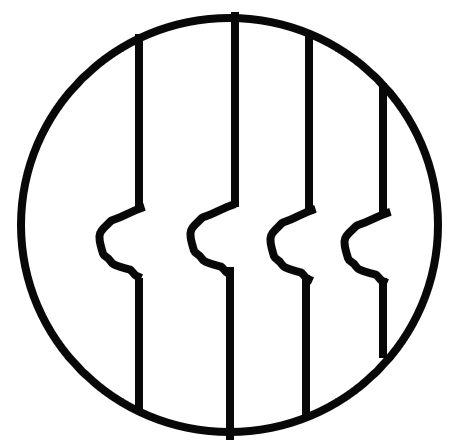
\includegraphics[width=0.3\textwidth]{20}}
		\subfigure{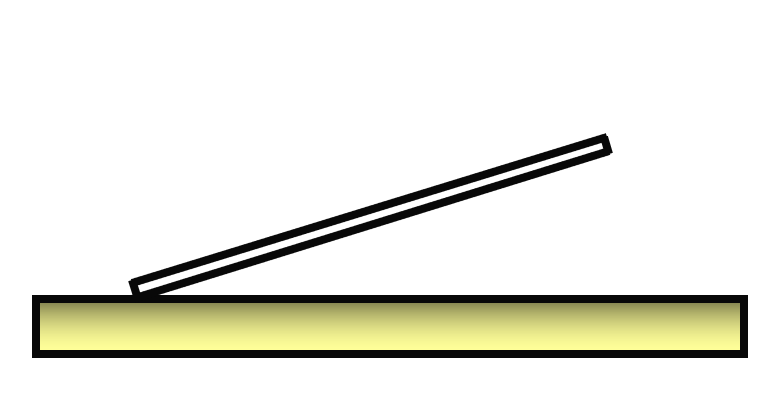
\includegraphics[width=0.3\textwidth]{21}}
	\end{figure}
\end{examples}
\begin{frame}
\frametitle{牛顿环}
\begin{figure}[!ht]
	\centering
	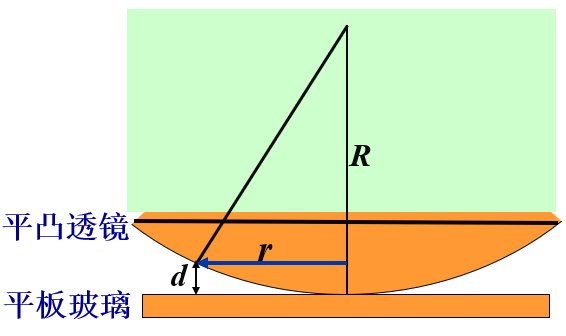
\includegraphics[width=0.5\textwidth]{22}
\end{figure}
\begin{block}{结论(考虑半波损失)}
	干涉环半径$r_{{k}}\approx\begin{cases}
			\sqrt{\frac{(2k-1)R\lambda}{2n}}\mathrm{~(k=1,2\cdots)}\quad\max\\\sqrt{kR\lambda/n}\mathrm{~(k=0,1\cdots)}\quad\min
		\end{cases}$
\end{block}
\end{frame}
\begin{frame}
	\frametitle{牛顿环条纹特征及动态变化}
	考虑半波损失的情况下
	\begin{figure}[!ht]
		\centering
		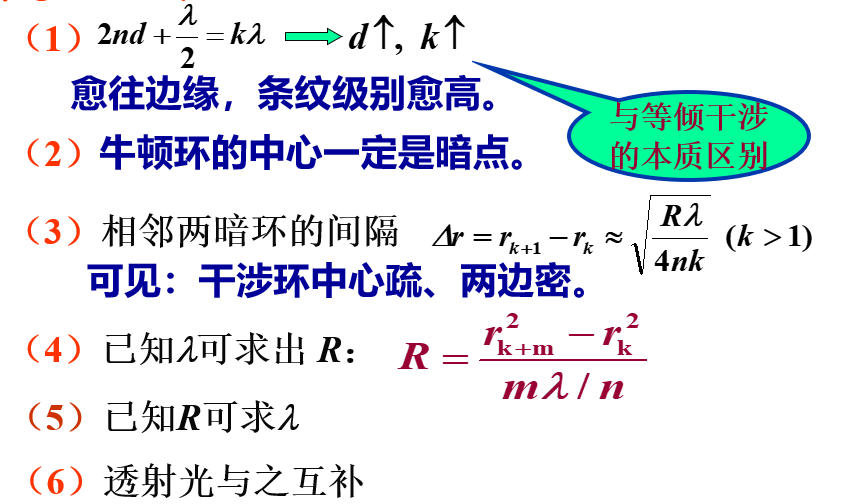
\includegraphics[width=0.8\textwidth]{23}
	\end{figure}
\end{frame}
\begin{frame}
\frametitle{迈克尔逊干涉仪}
	\begin{figure}[!ht]
	\centering
	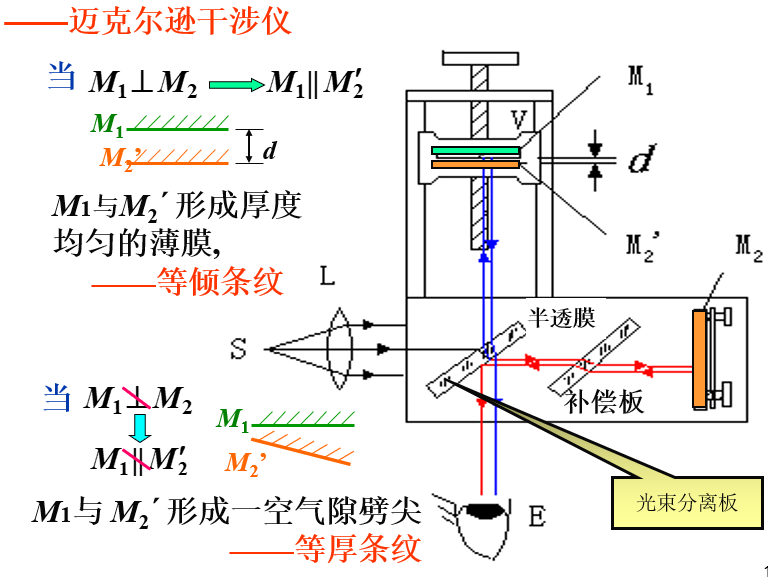
\includegraphics[width=0.8\textwidth]{30}
\end{figure}
\end{frame}

\begin{frame}
\frametitle{弗朗和费衍射}
惠更斯——菲涅耳原理:波传到的任何一点都是子波的波源,各子波在空间某点的相干叠加,就决定了该点波的强度。
\begin{figure}[!ht]
	\centering
	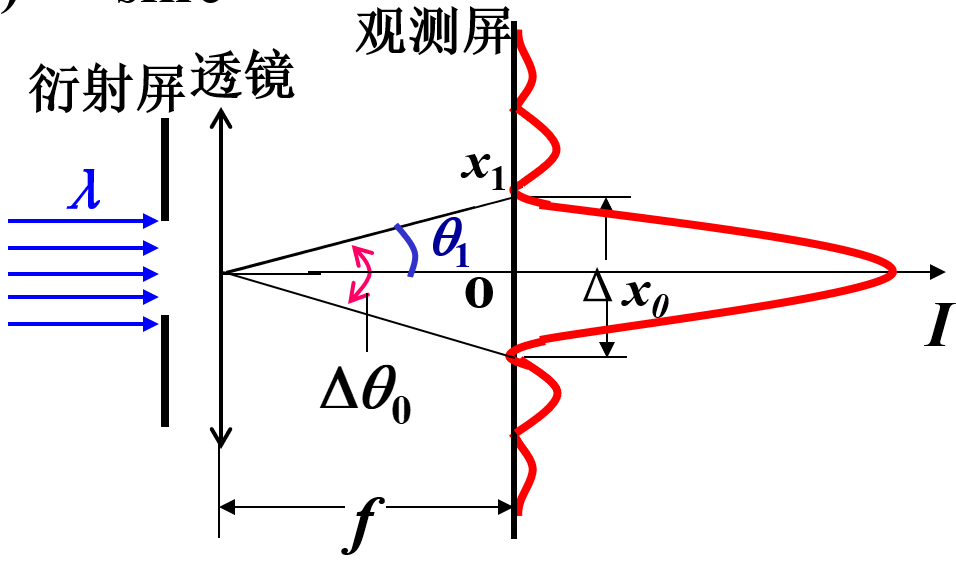
\includegraphics[width=0.5\textwidth]{24}
\end{figure}
\begin{block}{结论}
	$I_\theta=I_0\left(\frac{\sin \alpha}{\alpha}\right)^2$ 其中 $\alpha=\frac{\pi a \sin \theta}{\lambda}$
\end{block}
\end{frame}
\begin{frame}

	\begin{block}{结论}
		衍射极小: $a\sin\theta=\pm k\lambda $
		
		衍射次极大:$$a\sin\theta{=}\pm1.43\lambda,\pm2.46\lambda,\pm3.47\lambda,\cdotp\cdotp\cdotp\Rightarrow a\sin\theta{\approx}\pm(2k+1)\frac\lambda2$$
		
		中央明纹的线宽度: $\Delta x \approx 2 f \frac{\lambda}{a}$ 半角宽度: $\theta_1 \approx \frac{\lambda}{a}$
	\end{block}
	了解半波带法:$a\sin\theta=k\frac\lambda2$,k为波带数,每两个波带会相消
	\begin{examples}
		一束单色光垂直投射到宽度为$a=6.00\times10^{-1}mm$射在距缝 $D=4.00\times10cm$ 的屏上。距中央明纹中心距离为 $y=1.40mm$ 处是明条纹。求 (1)入射光的波长;(2)$y=1.40mm$ 处的条纹级数$k$ ; (3)根据所求得的级数$k$ , 计算此光波在狭缝处波阵面可作半波带的数目
	\end{examples}
\end{frame}
\begin{frame}
\frametitle{双缝衍射}
\begin{figure}[!ht]
	\centering
	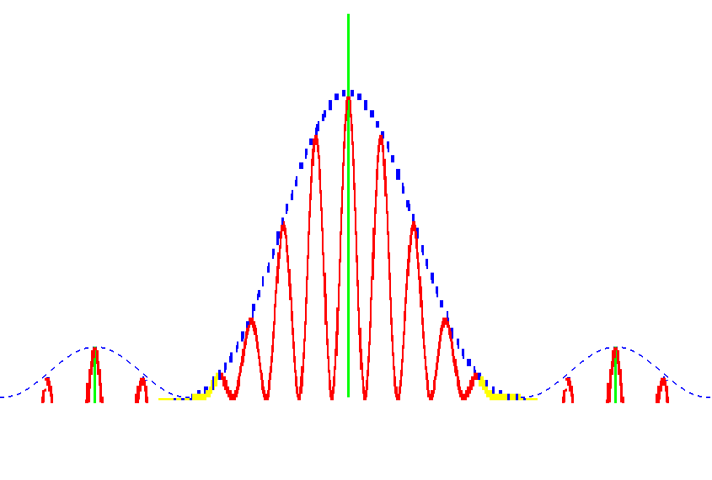
\includegraphics[width=0.7\textwidth]{31}
\end{figure}
$$
I_\theta=I_0\left(\frac{\sin \alpha}{\alpha}\right)^2 \cos ^2 \beta,\alpha=\frac{\pi a \sin \theta}{\lambda} ,\beta=\frac{\pi d \sin \theta}{\lambda}
$$
\end{frame}
\begin{frame}
	\frametitle{双缝衍射}
\begin{block}{双缝衍射光强度的分布规律}
衍射极小 $\quad a \sin \theta= \pm k \lambda \quad k=1,2, \cdots$

干涉极小: $\quad d \sin \theta= \pm\left(2 k^{\prime}+1\right) \frac{\lambda}{2}$

干涉极大: $\quad d \sin \theta= \pm k^{\prime} \lambda \quad k^{\prime}=0,1,2, \cdots$

若干涉极大同时衍射极小:$k^{\prime}=k \frac{d}{a}=$ 整数—缺级
\end{block}
\begin{examples}
	对于$d=0.15mm,a=0.030mm$的双缝,波长$\lambda=5.5\times10^{-7}m$ 的光入射。包络线的两个第一极小间有多少条完整条纹出现?
\end{examples}
\end{frame}
\begin{frame}
	\frametitle{光栅}
		\begin{figure}[!ht]
		\centering
		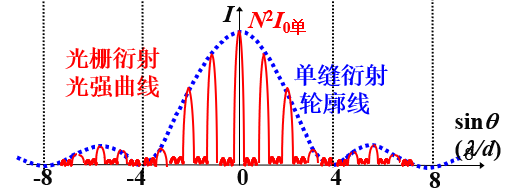
\includegraphics[width=0.8\textwidth]{25}
	\end{figure}
	亮线光栅强度分布: $I_\theta=I_0\left(\frac{\sin \alpha}{\alpha}\right)^2\left(\frac{\sin N \beta}{\sin \beta}\right)^2$
	
	主极大/明纹:$d \sin \theta=k \lambda, k=0, \pm 1, \pm 2, \ldots$
	
	暗纹:$d\sin\theta=\pm\frac{k^{\prime}}N\lambda=\pm(k+\frac mN)\lambda,k=0,1,..., m=1,2...N-1$

	存在缺项,与双缝衍射同理:衍射极小,干涉极大
\end{frame}
\begin{frame}
	\frametitle{光栅主极大的半角宽}
	\begin{figure}[!ht]
		\centering
		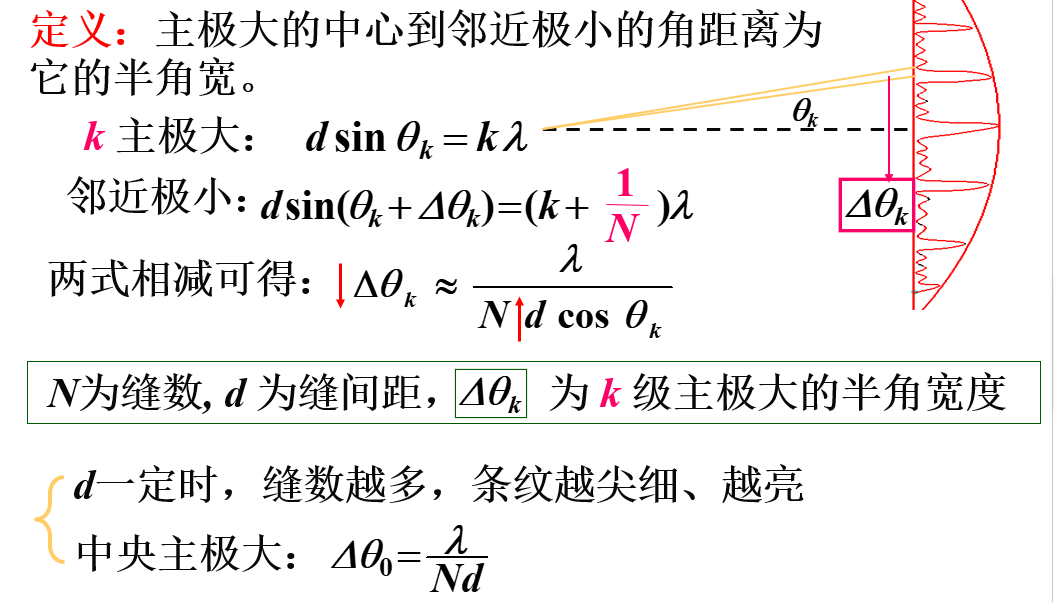
\includegraphics[width=0.9\textwidth]{32}
	\end{figure}

\end{frame}
\begin{frame}
	\frametitle{X 射线衍射与布喇格公式}
	\begin{figure}[!ht]
		\centering
		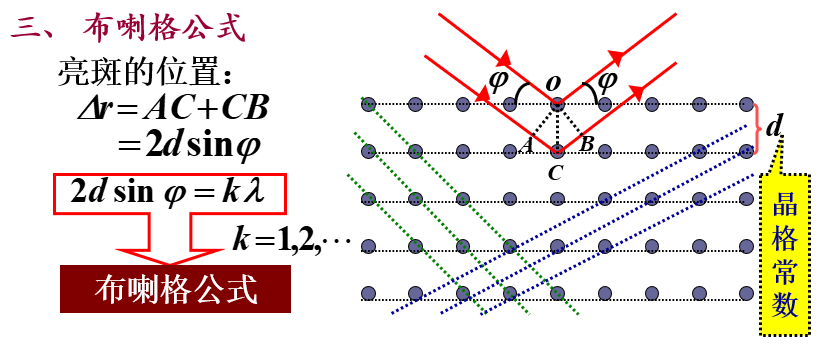
\includegraphics[width=0.8\textwidth]{26}
	\end{figure}
	考的可能性不大
\end{frame}
\begin{frame}
	\frametitle{圆孔衍射与光学仪器的分辨本领}
	\begin{figure}[!ht]
		\centering
		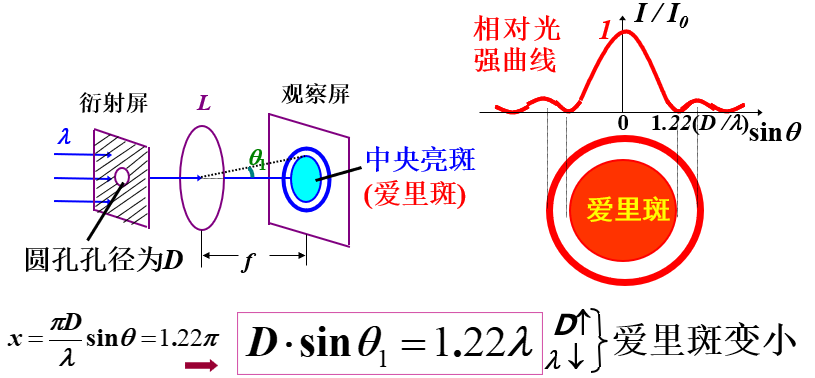
\includegraphics[width=0.8\textwidth]{27}
	\end{figure}
	光学仪器分辨率:
	${\theta}_{\lim}=\sin^{-1}\left(1.22\frac\lambda D\right)\boldsymbol{\approx}1.22\frac\lambda D$
	
	光栅光谱, 光栅的色散本领、分辨本领略
	
\end{frame}
\begin{frame}
\frametitle{马吕斯定律}
了解五种偏振光的分类
	\begin{figure}[!ht]
	\centering
	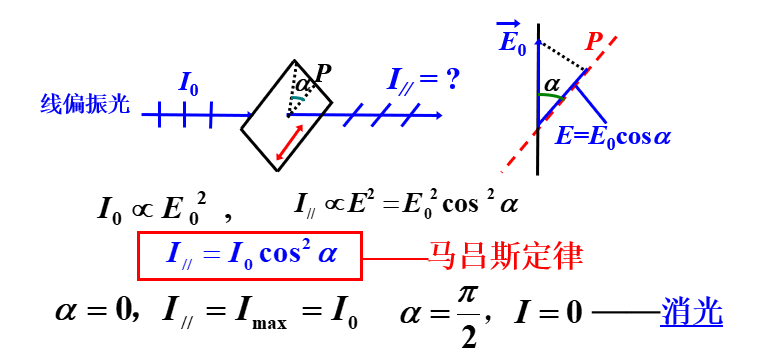
\includegraphics[width=0.7\textwidth]{28}
\end{figure}
\begin{examples}
	一束光由线偏振光和自然光混合而成,当它通过理想偏振片时,光强随偏振片偏振化方向旋转出现5倍变化,求这两种光比例?
\end{examples}
\end{frame}
\begin{frame}
	\frametitle{布儒斯特定律}

	布儒斯特定律:自然光以布儒斯特角入射到界面时,反射光为线偏振光
	\begin{figure}[!ht]
	\centering
	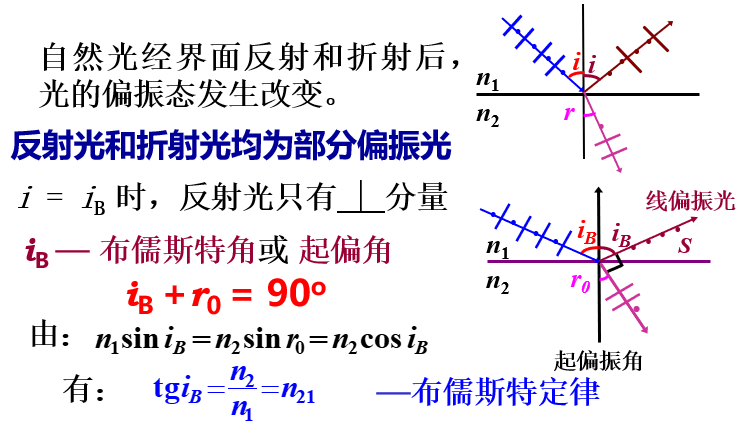
\includegraphics[width=0.8\textwidth]{29}
\end{figure}	

\end{frame}
\begin{frame}
	\frametitle{双折射}
一条入射光线产生两条折射光线(o光和e光)的现象
	\begin{figure}[!ht]
	\centering
	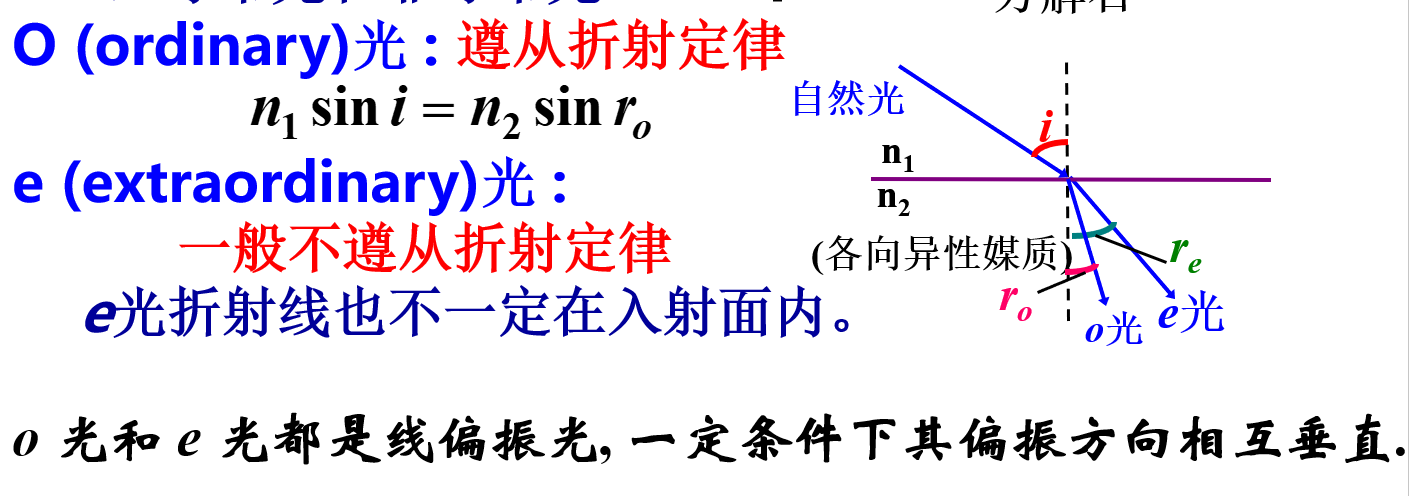
\includegraphics[width=0.8\textwidth]{33}
\end{figure}		
	波晶片(波片):o光和e光通过时,获得额外位相差获得椭圆偏振光:线偏振光通过 $\lambda / 4$ 波片
	
	会通过偏振片和波晶片检验光的类型,结合偏振知识,处理光的干涉问题。
\end{frame}
\begin{frame}
	\frametitle{双折射的惠更斯解释}
	\begin{figure}[!ht]
		\centering
		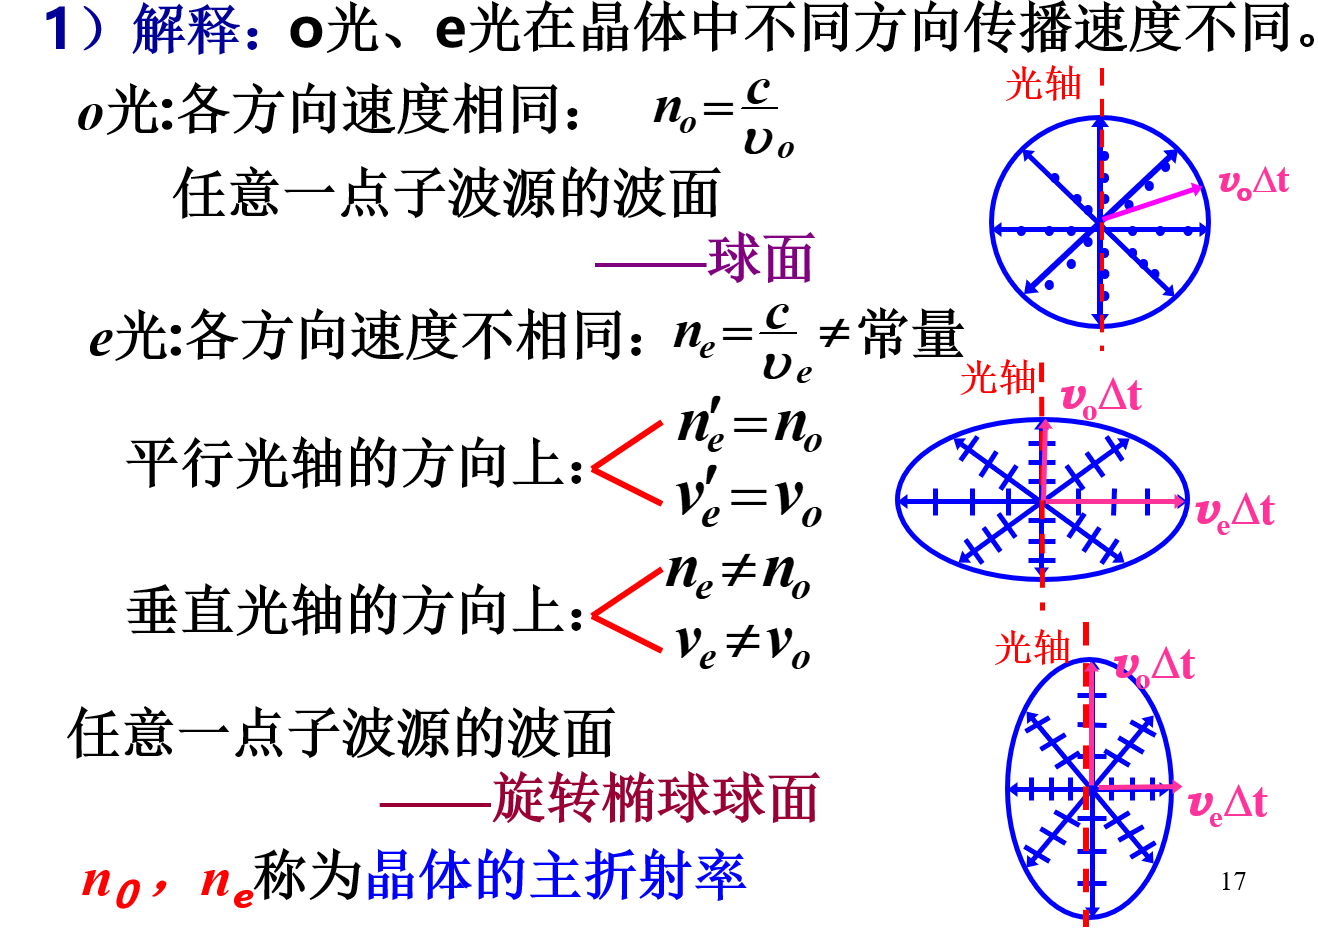
\includegraphics[width=0.8\textwidth]{34}
	\end{figure}		
	
\end{frame}
\begin{frame}
	\frametitle{双折射的惠更斯解释}
	\begin{figure}[!ht]
		\centering
		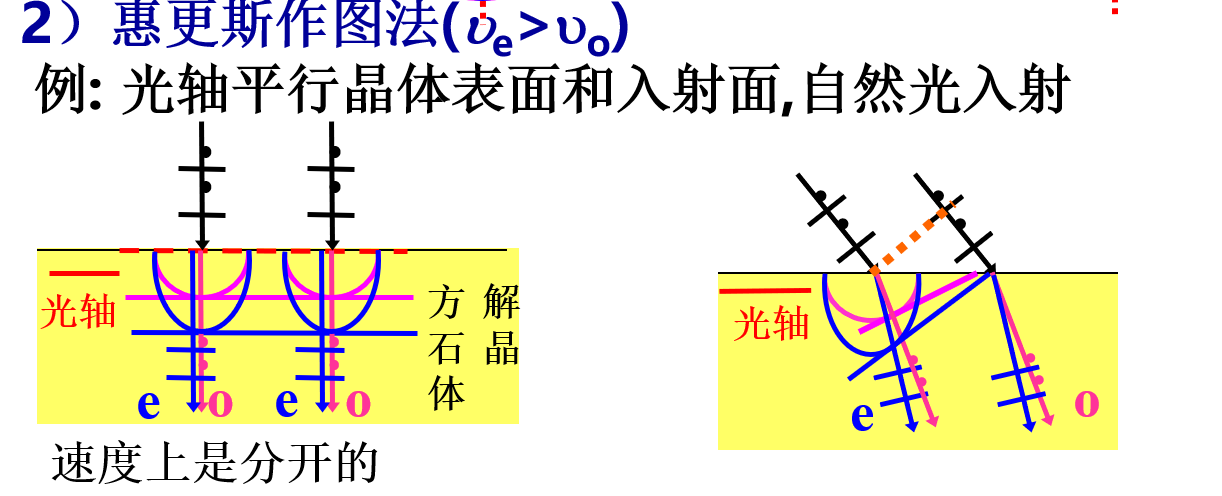
\includegraphics[width=1\textwidth]{35}
	\end{figure}		
\end{frame}
\begin{frame}
\frametitle{波晶片/相位延迟片}
波晶片是光轴平行表面的晶体薄片。

通过厚为d的晶片,o、e光不可分开,但产生光程差:$$\Delta r=l_{{o}}-l_{{e}}=d(n_o-n_{{e}})\Rightarrow \Delta\varphi=\frac{\Delta r}\lambda2\pi=(n_o-n_e)\cdot d\cdot\frac{2\pi}\lambda $$
	
可见:$\lambda$一定,适当选择$d$ 可使两分振动产生任意数值的位相差。
		
常用波片:$\begin{cases}
	\text{四分之一波片}&\Rightarrow|n_e-n_o|d=\frac{\lambda}{4},|\Delta \phi| = \frac{\pi}{2}\\
	\text{二分之一波片}&\Rightarrow|n_e-n_o|d=\frac{\lambda}{2}, |\Delta \phi| = {\pi}\\
	\text{全波片}&\Rightarrow|n_e-n_o|d={\lambda}, |\Delta \phi| = {2\pi}\\
\end{cases}$
	
\end{frame}
\begin{frame}
	\frametitle{圆偏振光(椭圆偏振光)的获得}
	\begin{figure}[!ht]
		\centering
		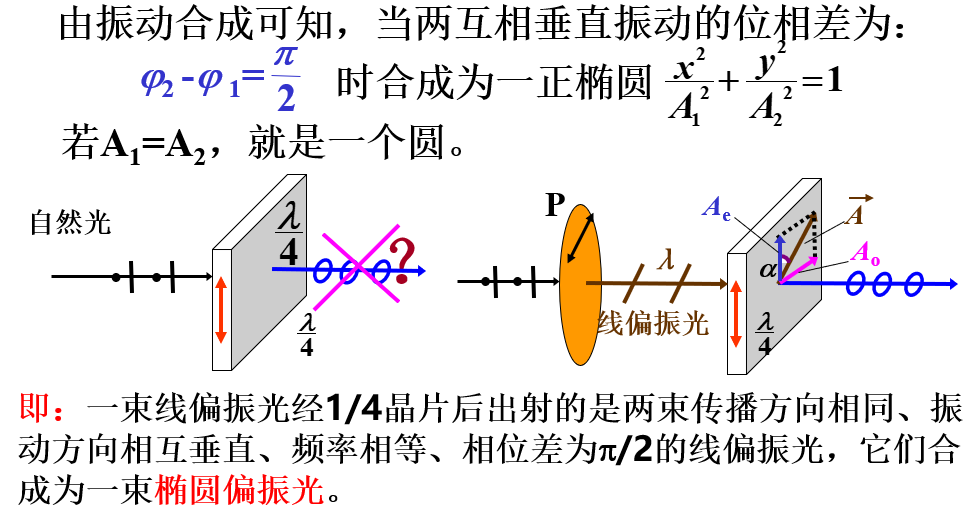
\includegraphics[width=1\textwidth]{36}
	\end{figure}
	不太理解的话原因的话可以看这个\href{https://www.bilibili.com/video/BV1Lt411t7Lh?vd_source=827e9d926cec44ef6817b376d985aae5}{\color{blue}{视频}}
\end{frame}
\begin{frame}

	\centering\Huge{\textbf{祝大家取得满意的成绩!}}		
\end{frame}
\end{document}